% kapitel5.tex
\chapter{Zusammenfassung}
\label{chapter:kap5}

\section{Reproduktion}
    Die Reproduktion von Gruppe 4 lief bei beiden Projekten gut. 
    
    \subsection{Projekt 1}
        \begin{itemize}
            \item Projekt war ausreichend kommentiert, strukturiert und Änderungen/Additionen klar sichtbar
            \item Code sowie grafische Darstellung ohne Probleme ausführbar
            \item Algorithmische Ideen auf Basis der Zwischenpräsentation gut umgesetzt
            \item Ergebnisse eigener Ausführung identisch mit originalen Ergebnissen
        \end{itemize}

        In Abbildung \ref{fig:reproduktion_project_1} sind die Ergebnisse unserer Reproduktion. Diese waren dieselben, wie bei denen.

        \begin{figure}
            \centering
            \begin{subfigure}{0.45\textwidth}
                \centering
                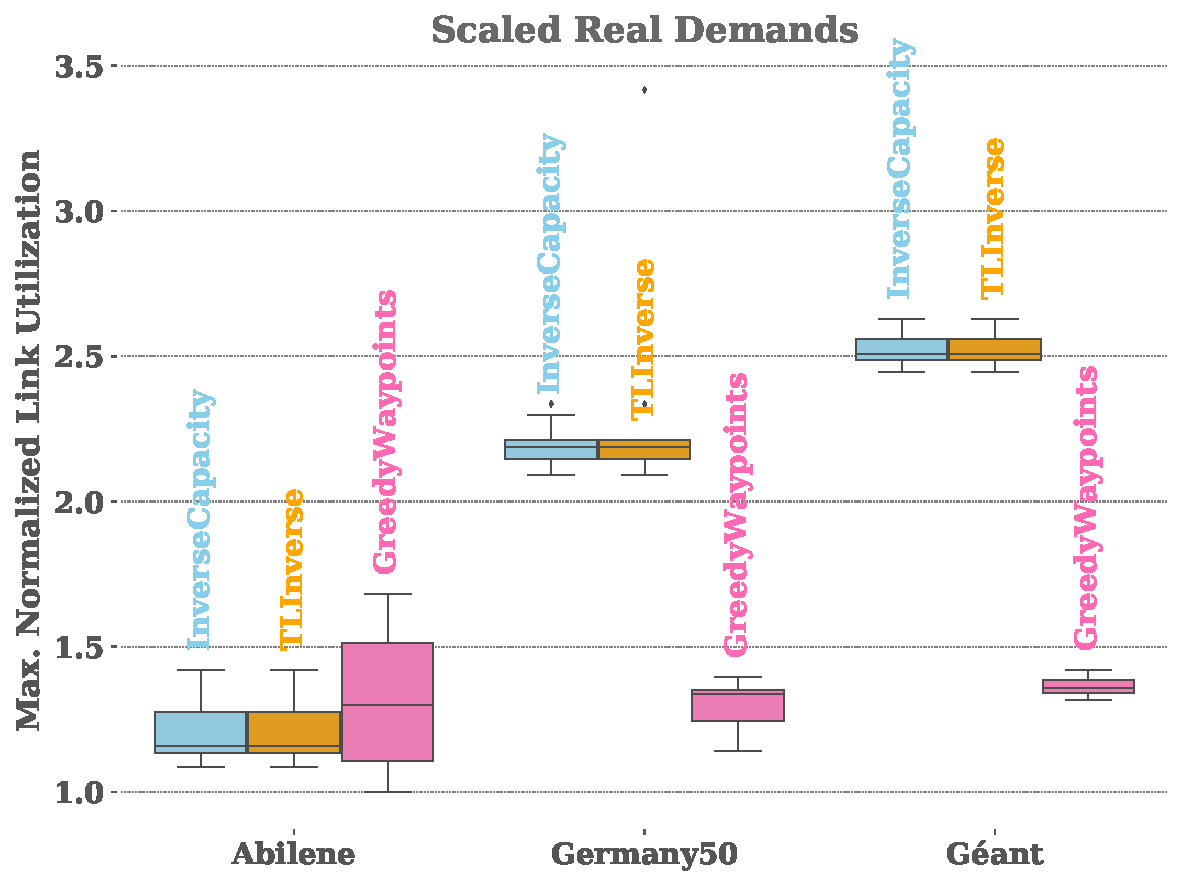
\includegraphics[width=1\linewidth]{Report/bilder/reproduktion/projekt1/real_demands alpha_0,3.pdf}
                \caption{Werte für $\alpha = 0.3$}
                \label{fig:reproduktion_project_1_a=0.3}
            \end{subfigure}
            \begin{subfigure}{0.45\textwidth}
                \centering
                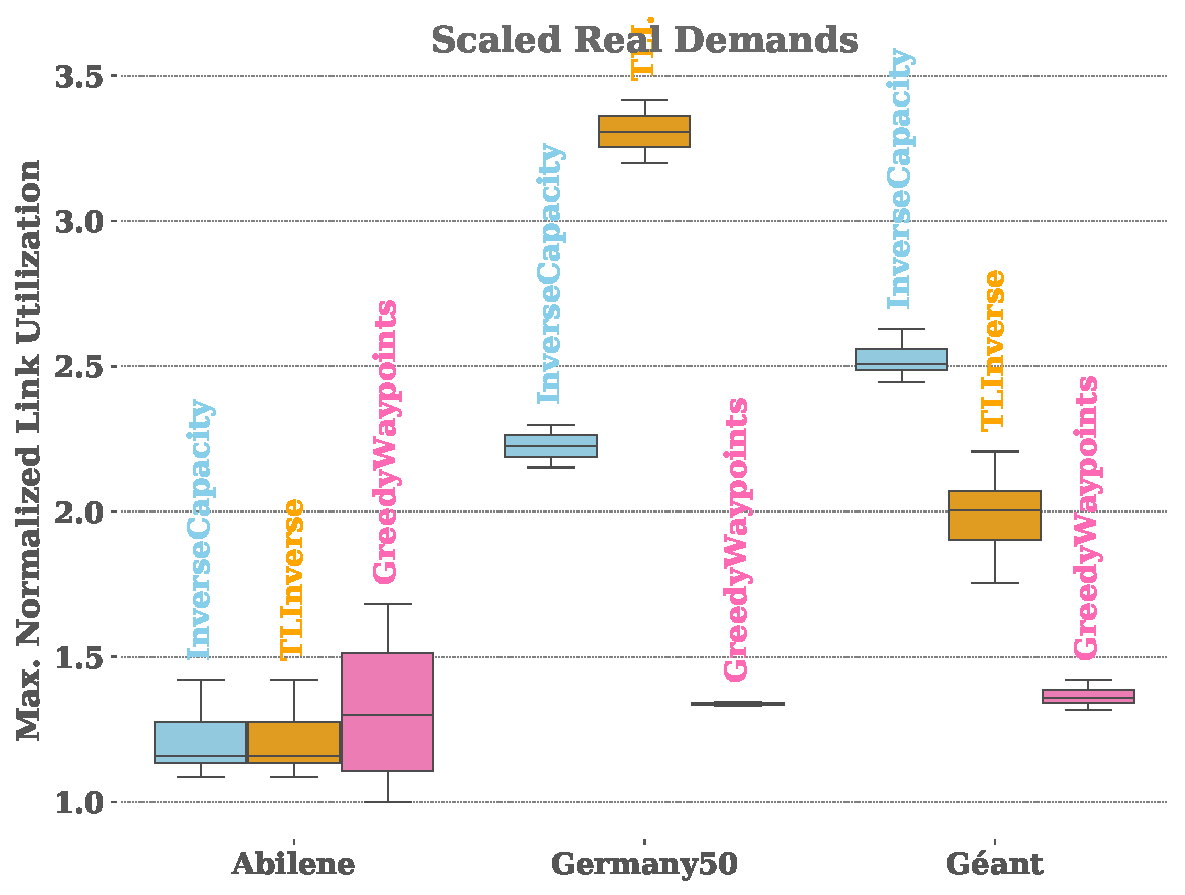
\includegraphics[width=1\linewidth]{Report/bilder/reproduktion/projekt1/real_demands alpha_0,5.pdf}
                \caption{Werte für $\alpha = 0.5$}
                \label{fig:reproduktion_project_1_a=0.5}
            \end{subfigure}
            \begin{subfigure}{0.45\textwidth}
                \centering
                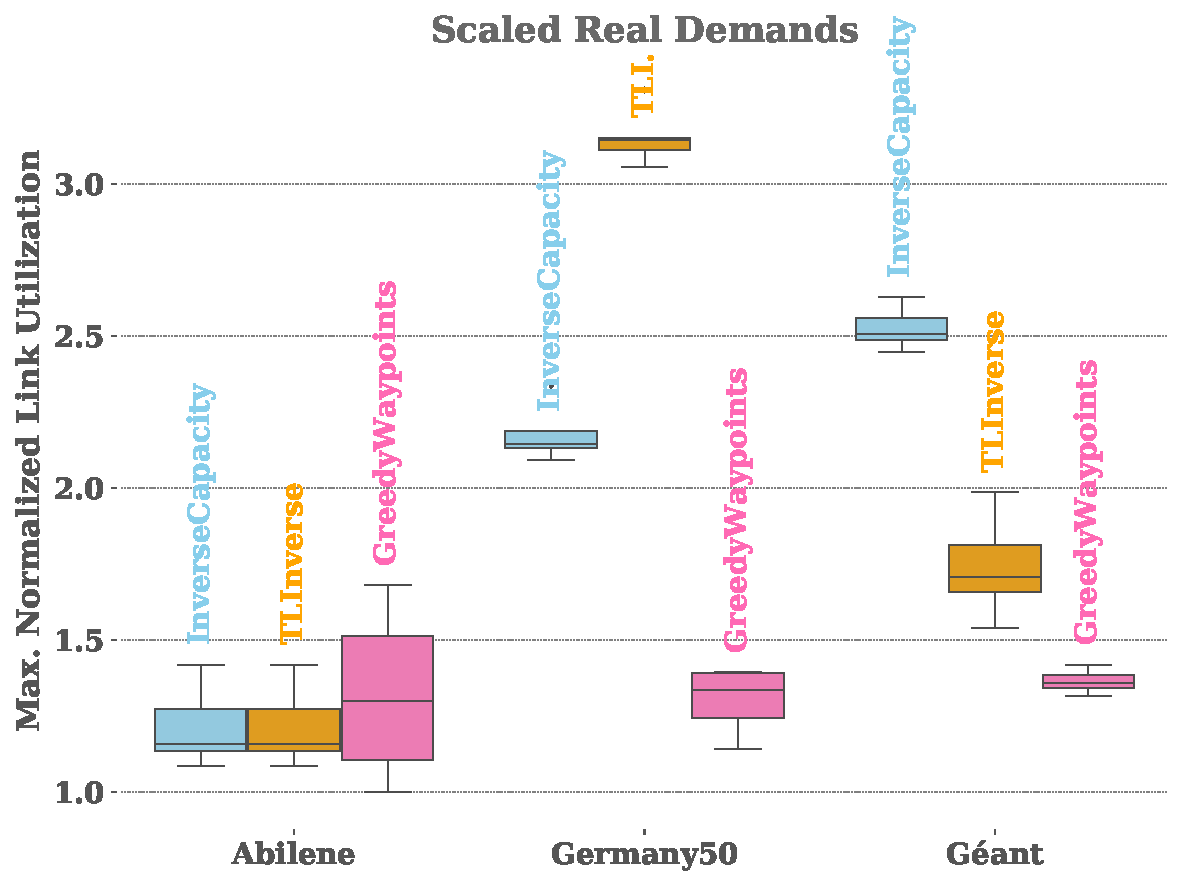
\includegraphics[width=1\linewidth]{Report/bilder/reproduktion/projekt1/real_demands alpha_0,7.pdf}
                \caption{Werte für $\alpha = 0.7$}
                \label{fig:reproduktion_project_1_a=0.7}
            \end{subfigure}
            \begin{subfigure}{0.45\textwidth}
                \centering
                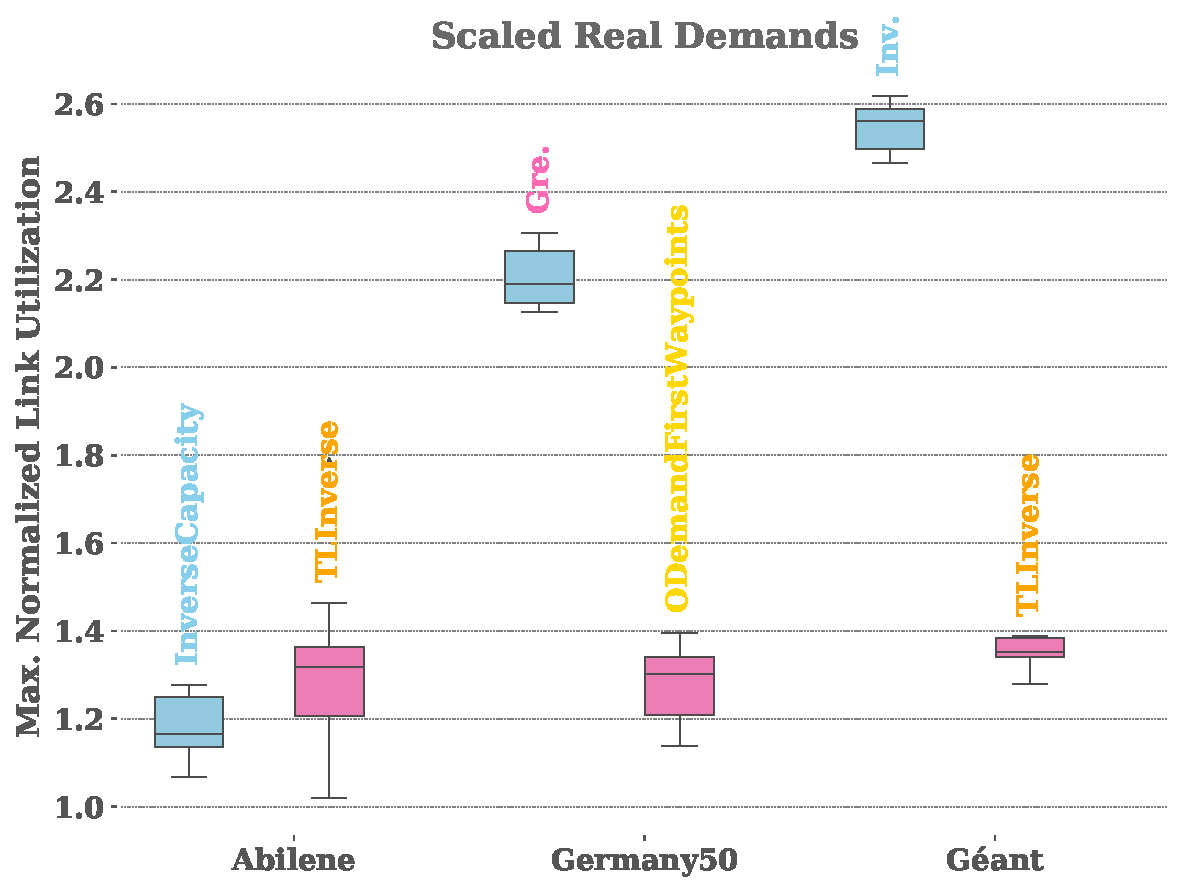
\includegraphics[width=1\linewidth]{Report/bilder/reproduktion/projekt1/real_demands.pdf}
                \caption{Werte für $\alpha = 1$}
                \label{fig:reproduktion_project_1_a=1}
            \end{subfigure}
            
            \caption{Reproduktion Projekt 1}
            \label{fig:reproduktion_project_1}
        \end{figure}

    \subsection{Projekt 2}

        \begin{itemize}
            \item Der Code lief ohne Probleme durch
            \item Unsere Ergebnisse sind aber aus irgendeinem Grund besser
            \begin{itemize}
                \item Vielleicht, weil mein Computer besser ist
            \end{itemize}
        \end{itemize}

        In Abbildung \ref{fig:reproduktion_project_2} sind unsere Reproduktionsergebnisse von Projekt zwei. Dabei sieht, dass das unsere Ergebnisse dabei besser abschneiden, als die von Gruppe 4. Zwischen den Ergebnissen aus \ref{fig:reproduktion_project_2_original_1} und \ref{fig:reproduktion_project_2_reproduktion_1} sind unsere Ergebnisse dabei 2- bis 5-mal so gut. Die Ergebnisse von \ref{fig:reproduktion_project_2_original_2} und \ref{fig:reproduktion_project_2_reproduktion_2} sind auch 2-mal so gut. Wobei scheint bei TL-Inverse aber ein Fehler aufgetreten.
        
        \begin{figure}
            \centering
            \begin{subfigure}{0.45\textwidth}
                \centering
                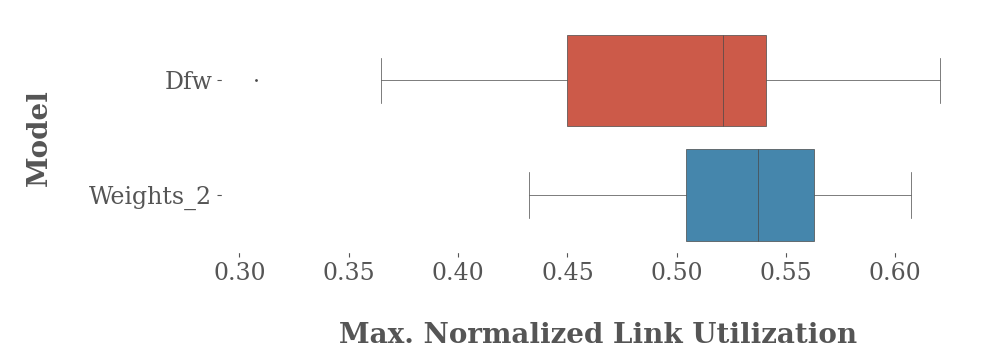
\includegraphics[width=1\linewidth]{Report/bilder/reproduktion/projekt2/original1.png}
                \caption{Original 1}
                \label{fig:reproduktion_project_2_original_1}
            \end{subfigure}
            \begin{subfigure}{0.45\textwidth}
                \centering
                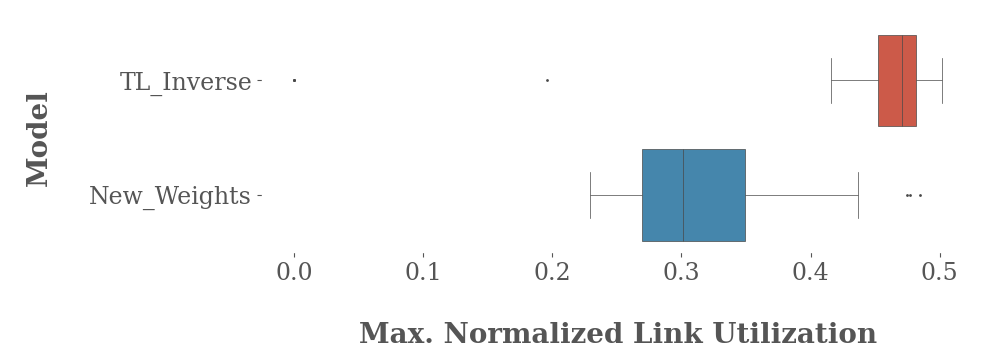
\includegraphics[width=1\linewidth]{Report/bilder/reproduktion/projekt2/original2.png}
                \caption{Original 2}
                \label{fig:reproduktion_project_2_original_2}
            \end{subfigure}
            \begin{subfigure}{0.45\textwidth}
                \centering
                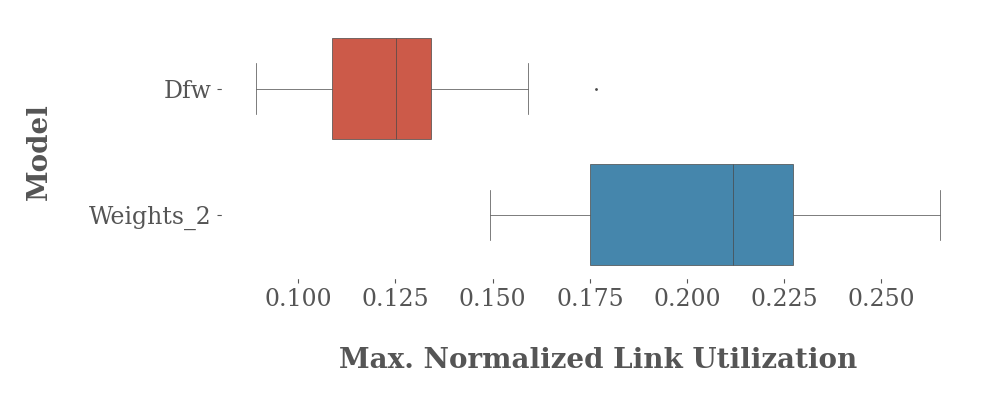
\includegraphics[width=1\linewidth]{Report/bilder/reproduktion/projekt2/reproduktion1.png}
                \caption{Reproduktion 1}
                \label{fig:reproduktion_project_2_reproduktion_1}
            \end{subfigure}
            \begin{subfigure}{0.45\textwidth}
                \centering
                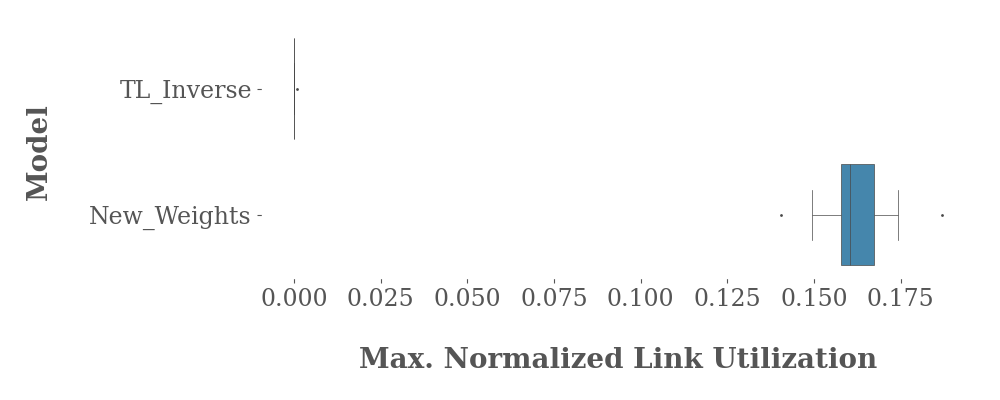
\includegraphics[width=1\linewidth]{Report/bilder/reproduktion/projekt2/reproduktion2.png}
                \caption{Reproduktion 2}
                \label{fig:reproduktion_project_2_reproduktion_2}
            \end{subfigure}
            
            \caption{Reproduktion Projekt 2}
            \label{fig:reproduktion_project_2}
        \end{figure}


\section{Fazit}
    Im Gesamten lief die Einarbeitung unserer Algorithmen gut. Es gab zwar an einigen Stellen Schwierigkeiten, sich in die Projekte einzuarbeiten und unsere Algorithmen passend zu implementieren, aber diese Schwierigkeiten konnten überwunden werden. Die Ergebnisse der Algorithmen waren dabei gemischt. Teilweise waren sie schneller als die schon existierenden Algorithmen, teilweise aber auch langsamer. Unsere Algorithmen haben sich dabei also gut in die schon existierenden aufgereiht. \\
    